% Created 2025-07-23 on 17:42
% Intended LaTeX compiler: pdflatex
\documentclass[12pt]{article}

%%%% settings when exporting code %%%% 

\usepackage{listings}
\lstdefinestyle{code-small}{
backgroundcolor=\color{white}, % background color for the code block
basicstyle=\ttfamily\small, % font used to display the code
commentstyle=\color[rgb]{0.5,0,0.5}, % color used to display comments in the code
keywordstyle=\color{black}, % color used to highlight certain words in the code
numberstyle=\ttfamily\tiny\color{gray}, % color used to display the line numbers
rulecolor=\color{black}, % color of the frame
stringstyle=\color[rgb]{0,.5,0},  % color used to display strings in the code
breakatwhitespace=false, % sets if automatic breaks should only happen at whitespace
breaklines=true, % sets automatic line breaking
columns=fullflexible,
frame=single, % adds a frame around the code (non,leftline,topline,bottomline,lines,single,shadowbox)
keepspaces=true, % % keeps spaces in text, useful for keeping indentation of code
literate={~}{$\sim$}{1}, % symbol properly display via latex
numbers=none, % where to put the line-numbers; possible values are (none, left, right)
numbersep=10pt, % how far the line-numbers are from the code
showspaces=false,
showstringspaces=false,
stepnumber=1, % the step between two line-numbers. If it's 1, each line will be numbered
tabsize=1,
xleftmargin=0cm,
emph={anova,apply,class,coef,colnames,colNames,colSums,dim,dcast,for,ggplot,head,if,ifelse,is.na,lapply,list.files,library,logLik,melt,plot,require,rowSums,sapply,setcolorder,setkey,str,summary,tapply},
aboveskip = \medskipamount, % define the space above displayed listings.
belowskip = \medskipamount, % define the space above displayed listings.
lineskip = 0pt} % specifies additional space between lines in listings
\lstset{style=code-small}
%%%% packages %%%%%

\usepackage[utf8]{inputenc}
\usepackage[T1]{fontenc}
\usepackage{lmodern}
\usepackage{textcomp}
\usepackage{color}
\usepackage{graphicx}
\usepackage{grffile}
\usepackage{wrapfig}
\usepackage{rotating}
\usepackage{longtable}
\usepackage{multirow}
\usepackage{multicol}
\usepackage{changes}
\usepackage{pdflscape}
\usepackage{geometry}
\usepackage[normalem]{ulem}
\usepackage{amssymb}
\usepackage{amsmath}
\usepackage{amsfonts}
\usepackage{dsfont}
\usepackage{array}
\usepackage{ifthen}
\usepackage{hyperref}
\usepackage{natbib}
\RequirePackage{setspace} % to modify the space between lines - incompatible with footnote in beamer
\renewcommand{\baselinestretch}{1.1}
\geometry{a4paper, left=10mm, right=10mm, top=10mm}
\usepackage{titlesec}
\usepackage{etoolbox}

\makeatletter
\patchcmd{\ttlh@hang}{\parindent\z@}{\parindent\z@\leavevmode}{}{}
\patchcmd{\ttlh@hang}{\noindent}{}{}{}
\makeatother
\RequirePackage{colortbl} % arrayrulecolor to mix colors
\definecolor{myorange}{rgb}{1,0.2,0}
\definecolor{mypurple}{rgb}{0.7,0,8}
\definecolor{mycyan}{rgb}{0,0.6,0.6}
\newcommand{\lightblue}{blue!50!white}
\newcommand{\darkblue}{blue!80!black}
\newcommand{\darkgreen}{green!50!black}
\newcommand{\darkred}{red!50!black}
\definecolor{gray}{gray}{0.5}
\hypersetup{
citecolor=[rgb]{0,0.5,0},
urlcolor=[rgb]{0,0,0.5},
linkcolor=[rgb]{0,0,0.5},
}
\newenvironment{note}{\small \color{gray}\fontfamily{lmtt}\selectfont}{\par}
\newenvironment{activity}{\color{orange}\fontfamily{qzc}\selectfont}{\par}
\RequirePackage{pifont}
\RequirePackage{relsize}
\newcommand{\Cross}{{\raisebox{-0.5ex}%
{\relsize{1.5}\ding{56}}}\hspace{1pt} }
\newcommand{\Valid}{{\raisebox{-0.5ex}%
{\relsize{1.5}\ding{52}}}\hspace{1pt} }
\newcommand{\CrossR}{ \textcolor{red}{\Cross} }
\newcommand{\ValidV}{ \textcolor{green}{\Valid} }
\usepackage{stackengine}
\usepackage{scalerel}
\newcommand\Warning[1][3ex]{%
\renewcommand\stacktype{L}%
\scaleto{\stackon[1.3pt]{\color{red}$\triangle$}{\tiny\bfseries !}}{#1}%
\xspace
}
\definecolor{grayR}{HTML}{8A8990}
\definecolor{grayL}{HTML}{C4C7C9}
\definecolor{blueM}{HTML}{1F63B5}
\newcommand{\Rlogo}[1][0.07]{
\begin{tikzpicture}[scale=#1]
\shade [right color=grayR,left color=grayL,shading angle=60]
(-3.55,0.3) .. controls (-3.55,1.75)
and (-1.9,2.7) .. (0,2.7) .. controls (2.05,2.7)
and (3.5,1.6) .. (3.5,0.3) .. controls (3.5,-1.2)
and (1.55,-2) .. (0,-2) .. controls (-2.3,-2)
and (-3.55,-0.75) .. cycle;

\fill[white]
(-2.15,0.2) .. controls (-2.15,1.2)
and (-0.7,1.8) .. (0.5,1.8) .. controls (2.2,1.8)
and (3.1,1.2) .. (3.1,0.2) .. controls (3.1,-0.75)
and (2.4,-1.45) .. (0.5,-1.45) .. controls (-1.1,-1.45)
and (-2.15,-0.7) .. cycle;

\fill[blueM]
(1.75,1.25) -- (-0.65,1.25) -- (-0.65,-2.75) -- (0.55,-2.75) -- (0.55,-1.15) --
(0.95,-1.15)  .. controls (1.15,-1.15)
and (1.5,-1.9) .. (1.9,-2.75) -- (3.25,-2.75)  .. controls (2.2,-1)
and (2.5,-1.2) .. (1.8,-0.95) .. controls (2.6,-0.9)
and (2.85,-0.35) .. (2.85,0.2) .. controls (2.85,0.7)
and (2.5,1.2) .. cycle;

\fill[white]  (1.4,0.4) -- (0.55,0.4) -- (0.55,-0.3) -- (1.4,-0.3).. controls (1.75,-0.3)
and (1.75,0.4) .. cycle;

\end{tikzpicture}
}
\RequirePackage{fancyvrb}
\DefineVerbatimEnvironment{verbatim}{Verbatim}{fontsize=\small,formatcom = {\color[rgb]{0.5,0,0}}}
\RequirePackage{enumitem} % better than enumerate
\RequirePackage{epstopdf} % to be able to convert .eps to .pdf image files
\RequirePackage{capt-of} %
\RequirePackage{caption} % newlines in graphics
\RequirePackage{tikz-cd} % graph
\RequirePackage{booktabs} % for nice lines in table (e.g. toprule, bottomrule, midrule, cmidrule)
\RequirePackage{amsmath}
\RequirePackage{algorithm}
\RequirePackage[noend]{algpseudocode}
\RequirePackage{dsfont}
\RequirePackage{amsmath,stmaryrd,graphicx}
\RequirePackage{prodint} % product integral symbol (\PRODI)
\usepackage{ifthen}
\usepackage{xifthen}
\usepackage{xargs}
\usepackage{xspace}
\newcommand\defOperator[7]{%
\ifthenelse{\isempty{#2}}{
\ifthenelse{\isempty{#1}}{#7{#3}#4}{#7{#3}#4 \left#5 #1 \right#6}
}{
\ifthenelse{\isempty{#1}}{#7{#3}#4_{#2}}{#7{#3}#4_{#1}\left#5 #2 \right#6}
}
}
\newcommand\defUOperator[5]{%
\ifthenelse{\isempty{#1}}{
#5\left#3 #2 \right#4
}{
\ifthenelse{\isempty{#2}}{\underset{#1}{\operatornamewithlimits{#5}}}{
\underset{#1}{\operatornamewithlimits{#5}}\left#3 #2 \right#4}
}
}
\newcommand{\defBoldVar}[2]{
\ifthenelse{\equal{#2}{T}}{\boldsymbol{#1}}{\mathbf{#1}}
}
\newcommandx\Esp[2][1=,2=]{\defOperator{#1}{#2}{E}{}{\lbrack}{\rbrack}{\mathbb}}
\newcommandx\Prob[2][1=,2=]{\defOperator{#1}{#2}{P}{}{\lbrack}{\rbrack}{\mathbb}}
\newcommandx\Qrob[2][1=,2=]{\defOperator{#1}{#2}{Q}{}{\lbrack}{\rbrack}{\mathbb}}
\newcommandx\Var[2][1=,2=]{\defOperator{#1}{#2}{V}{ar}{\lbrack}{\rbrack}{\mathbb}}
\newcommandx\Cov[2][1=,2=]{\defOperator{#1}{#2}{C}{ov}{\lbrack}{\rbrack}{\mathbb}}
\newcommandx\Binom[2][1=,2=]{\defOperator{#1}{#2}{B}{}{(}{)}{\mathcal}}
\newcommandx\Gaus[2][1=,2=]{\defOperator{#1}{#2}{N}{}{(}{)}{\mathcal}}
\newcommandx\Wishart[2][1=,2=]{\defOperator{#1}{#2}{W}{ishart}{(}{)}{\mathcal}}
\newcommandx\Likelihood[2][1=,2=]{\defOperator{#1}{#2}{L}{}{(}{)}{\mathcal}}
\newcommandx\logLikelihood[2][1=,2=]{\defOperator{#1}{#2}{\ell}{}{(}{)}{}}
\newcommandx\Information[2][1=,2=]{\defOperator{#1}{#2}{I}{}{(}{)}{\mathcal}}
\newcommandx\Score[2][1=,2=]{\defOperator{#1}{#2}{S}{}{(}{)}{\mathcal}}
\newcommandx\Vois[2][1=,2=]{\defOperator{#1}{#2}{V}{}{(}{)}{\mathcal}}
\newcommandx\IF[2][1=,2=]{\defOperator{#1}{#2}{IF}{}{(}{)}{\mathcal}}
\newcommandx\Ind[1][1=]{\defOperator{}{#1}{1}{}{(}{)}{\mathds}}
\newcommandx\Max[2][1=,2=]{\defUOperator{#1}{#2}{(}{)}{min}}
\newcommandx\Min[2][1=,2=]{\defUOperator{#1}{#2}{(}{)}{max}}
\newcommandx\argMax[2][1=,2=]{\defUOperator{#1}{#2}{(}{)}{argmax}}
\newcommandx\argMin[2][1=,2=]{\defUOperator{#1}{#2}{(}{)}{argmin}}
\newcommandx\cvD[2][1=D,2=n \rightarrow \infty]{\xrightarrow[#2]{#1}}
\newcommandx\Hypothesis[2][1=,2=]{
\ifthenelse{\isempty{#1}}{
\mathcal{H}
}{
\ifthenelse{\isempty{#2}}{
\mathcal{H}_{#1}
}{
\mathcal{H}^{(#2)}_{#1}
}
}
}
\newcommandx\dpartial[4][1=,2=,3=,4=\partial]{
\ifthenelse{\isempty{#3}}{
\frac{#4 #1}{#4 #2}
}{
\left.\frac{#4 #1}{#4 #2}\right\rvert_{#3}
}
}
\newcommandx\dTpartial[3][1=,2=,3=]{\dpartial[#1][#2][#3][d]}
\newcommandx\ddpartial[3][1=,2=,3=]{
\ifthenelse{\isempty{#3}}{
\frac{\partial^{2} #1}{\partial #2^2}
}{
\frac{\partial^2 #1}{\partial #2\partial #3}
}
}
\newcommand\Real{\mathbb{R}}
\newcommand\Rational{\mathbb{Q}}
\newcommand\Natural{\mathbb{N}}
\newcommand\trans[1]{{#1}^\intercal}%\newcommand\trans[1]{{\vphantom{#1}}^\top{#1}}
\newcommand{\independent}{\mathrel{\text{\scalebox{1.5}{$\perp\mkern-10mu\perp$}}}}
\newcommand\half{\frac{1}{2}}
\newcommand\normMax[1]{\left|\left|#1\right|\right|_{max}}
\newcommand\normTwo[1]{\left|\left|#1\right|\right|_{2}}
\newcommand\Veta{\boldsymbol{\eta}}
\newcommand\VX{\mathbf{X}}
\author{Brice Ozenne}
\date{\today}
\title{Performing GPC in a paired design}
\hypersetup{
 colorlinks=true,
 pdfauthor={Brice Ozenne},
 pdftitle={Performing GPC in a paired design},
 pdfkeywords={},
 pdfsubject={},
 pdfcreator={Emacs 30.1 (Org mode 9.7.11)},
 pdflang={English}
 }
\begin{document}

\maketitle
This vignette describes how to use Generalized Pairwise comparisons
(GPC) in a paired design. This for instance corresponds to the
Diabetic Retinopathy Study (DRS) contained in the survival \Rlogo
package where 197 patients had one of their eye randomized to laser
treatment while the other did not receive any treatment:
\begin{lstlisting}[language=r,numbers=none]
data(diabetic, package = "survival")
head(diabetic)
\end{lstlisting}

\phantomsection
\label{}
\begin{verbatim}
  id laser age   eye trt risk  time status
1  5 argon  28  left   0    9 46.23      0
2  5 argon  28 right   1    9 46.23      0
3 14 xenon  12  left   1    8 42.50      0
4 14 xenon  12 right   0    6 31.30      1
5 16 xenon   9  left   1   11 42.27      0
6 16 xenon   9 right   0   11 42.27      0
\end{verbatim}


The outcome was time to blindness (visual acuity drop below a certain
threshold). In the real study \texttt{status} equal to 0 mixes death and
censoring (due to drop-out or end of study) but this complication will
be neglected here for simplicity.


\bigskip

We will replicate some of the analyzes presented in
\cite{matsouaka2022robust}. In this paper they split the dataset into
juvenile and adult patients:
\begin{lstlisting}[language=r,numbers=none]
diabetic$juvenile <- diabetic$age <= 19
library(LMMstar)
summarize(age ~ juvenile, data = diabetic[!duplicated(diabetic$id),])
\end{lstlisting}

\phantomsection
\label{}
\begin{verbatim}
  juvenile observed missing     mean        sd min q1 median    q3 max
1    FALSE       83       0 35.30120 11.242054  20 25     34 45.00  58
2     TRUE      114       0 10.21053  4.713892   1  7     10 13.75  19
\end{verbatim}


and we will focus on the juvenile patients:
\begin{lstlisting}[language=r,numbers=none]
diabeticJ <- diabetic[diabetic$juvenile,]
\end{lstlisting}

\clearpage
\section{Wald methods (Gehan scoring rule)}
\label{sec:org35a98d4}

To mimic the methodology underlying the results presented in Table 1
of \cite{matsouaka2022robust}, we perform GPC stratified by patient
using the Gehan scoring rule:
\begin{lstlisting}[language=r,numbers=none]
library(BuyseTest)
e.BTjuv <- BuyseTest(trt ~ tte(time,status) + strata(id, match = TRUE), 
                     data = diabeticJ, trace = FALSE,
                     scoring.rule =  "Gehan")
model.tables(e.BTjuv, percentage = FALSE)
\end{lstlisting}

\phantomsection
\label{}
\begin{verbatim}
  endpoint total favorable unfavorable neutral uninf     Delta   lower.ci  upper.ci    p.value
1     time   114        39          21       3    51 0.1578947 0.02591623 0.2844633 0.01922741
\end{verbatim}


Indeed this scoring rule does not involve any extra-modeling, only
evaluating the patient specific net benefit and averaging them:
\begin{lstlisting}[language=r,numbers=none]
mean(coef(e.BTjuv, strata = TRUE))
\end{lstlisting}

\phantomsection
\label{}
\begin{verbatim}
[1] 0.1578947
\end{verbatim}


\cite{matsouaka2022robust} propose to estimate the standard error as:
\begin{lstlisting}[language=r,numbers=none]
N <- nobs(e.BTjuv)["pairs"]
pw <- coef(e.BTjuv, statistic = "favorable")
pl <- coef(e.BTjuv, statistic = "unfavorable")
sqrt((pw + pl - (pw - pl)^2)/N)
\end{lstlisting}

\phantomsection
\label{}
\begin{verbatim}
      time 
0.06631828
\end{verbatim}


which matches what \texttt{BuyseTest} output:
\begin{lstlisting}[language=r,numbers=none]
confint(e.BTjuv)
\end{lstlisting}

\phantomsection
\label{}
\begin{verbatim}
      estimate         se   lower.ci  upper.ci null    p.value
time 0.1578947 0.06631828 0.02591623 0.2844633    0 0.01922741
\end{verbatim}


By default \texttt{confint} uses a hyperbolic tangent to compute confidence
intervals (CIs), which will then differ from the 'Wald' discussed in
\cite{matsouaka2022robust}. These 'untransformed Wald' CIs can be
retrieved by setting the argument \texttt{transform} to \texttt{FALSE}:
\begin{lstlisting}[language=r,numbers=none]
confint(e.BTjuv, transform = FALSE)
\end{lstlisting}

\phantomsection
\label{}
\begin{verbatim}
      estimate         se   lower.ci  upper.ci null    p.value
time 0.1578947 0.06631828 0.02791329 0.2878762    0 0.01727214
\end{verbatim}


\clearpage

\uline{Note:} naively one may think to estimate the standard error as:
\begin{lstlisting}[language=r,numbers=none]
sqrt(var(coef(e.BTjuv, strata = TRUE))/N)
\end{lstlisting}

\phantomsection
\label{}
\begin{verbatim}
     pairs 
0.06661108
\end{verbatim}


This is equivalent (in large samples to the previous formula). Indeed:
\begin{align*}
&\Prob[X>Y] + \Prob[Y>X] - (\Prob[X>Y] - \Prob[Y>X])^2 \\
=& \Prob[X>Y] + \Prob[Y>X] - \Prob[X>Y]^ - \Prob[Y>X]^2 + 2 \Prob[X>Y] \Prob[Y>X] \\
=& \Prob[X>Y](1-\Prob[X>Y]) + \Prob[Y>X](1-\Prob[Y>X]) + 2 \Prob[X>Y] \Prob[Y>X] \\
=& \Prob[X>Y](1-\Prob[X>Y]) + \Prob[Y>X](1-\Prob[Y>X]) \\
 & - 2 (0 - \Prob[X>Y] \Prob[Y>X] - \Prob[X>Y] \Prob[Y>X] + \Prob[X>Y] \Prob[Y>X] \\
=& \Var\left[\Ind[X>Y]\right] + \Var\left[\Ind[X<Y]\right] - 2 \Cov\left(\Ind[X>Y],\Ind[X<Y]\right) \\
=& \Var\left[\Ind[X>Y]-\Ind[X<Y]\right] \\
\end{align*}

There is only a factor \texttt{N/(N-1)} difference between the two:
\begin{lstlisting}[language=r,numbers=none]
sqrt(var(coef(e.BTjuv, strata = TRUE))/N) * sqrt((N-1)/N)
\end{lstlisting}

\phantomsection
\label{}
\begin{verbatim}
     pairs 
0.06631828
\end{verbatim}
\section{MOVER method (Gehan scoring rule)}
\label{sec:org121445d}

The method recommended by \cite{matsouaka2022robust} is the MOVER
approach, which has been developped for a binary scoring rule
(e.g. Gehan). An experimental function with the same name has been
implemented in the BuyseTest package:

\begin{lstlisting}[language=r,numbers=none]
BuyseTest:::mover(e.BTjuv)
\end{lstlisting}
\phantomsection
\label{}
\begin{verbatim}
  estimate      lower      upper     pvalue 
0.15789474 0.02540421 0.28317729 0.01967878
\end{verbatim}


leading to the same results as those of the table 1 in the original article, up to rounding.

\clearpage
\section{Wald methods (Peron scoring rule)}
\label{sec:org94f1d11}

To better account for censoring one could use the Peron scoring rule
where the survival is estimated across all subjects within a treatment
group. One has to specify the survival model, otherwise, the BuyseTest
function will estimate a treatmnet and strata specific survival curve
which is impossible to perform here. The \texttt{model.tte} argument can be
used to specify such survival model:
\begin{lstlisting}[language=r,numbers=none]
library(prodlim)
e.BTjuv2 <- BuyseTest(trt ~ tte(time,status) + strata(id, match = TRUE), 
                      data = diabeticJ, trace = FALSE,
                      model.tte = prodlim(Hist(time,status)~ trt, data = diabeticJ))
model.tables(e.BTjuv2, percentage = FALSE)
\end{lstlisting}

\phantomsection
\label{}
\begin{verbatim}
  endpoint total favorable unfavorable neutral    uninf    Delta   lower.ci  upper.ci
1     time   114  47.36525    24.29552       3 39.33923 0.202366 0.05045454 0.3451254
      p.value
1 0.009329589
\end{verbatim}


Ignoring the uncertainty of the survival model, the standard would be:
\begin{lstlisting}[language=r,numbers=none]
c(sqrt(var(coef(e.BTjuv2, strata = TRUE))/N),
  sqrt(var(coef(e.BTjuv2, strata = TRUE))/N) * sqrt((N-1)/N)
  )
\end{lstlisting}

\phantomsection
\label{}
\begin{verbatim}
     pairs      pairs 
0.06595510 0.06566518
\end{verbatim}


depending on whether a small sample correction is used or not. This
matches the output of \texttt{BuyseTest} when ignoring the uncertainty of the
survival model:
\begin{lstlisting}[language=r,numbers=none]
model.tte <- prodlim(Hist(time,status)~ trt, data = diabeticJ)
attr(model.tte, "iidNuisance") <- FALSE
confint(BuyseTest(trt ~ tte(time,status) + strata(id, match = TRUE), 
                  data = diabeticJ, trace = FALSE,
                  model.tte = model.tte))
\end{lstlisting}

\phantomsection
\label{}
\begin{verbatim}
     estimate         se   lower.ci  upper.ci null     p.value
time 0.202366 0.06566518 0.07088227 0.3269375    0 0.002726979
\end{verbatim}


\Warning Because the pairwise win and loss score are no more binary, the
previous formula no more simplifies into the formula presented in
\cite{matsouaka2022robust}:
\begin{lstlisting}[language=r,numbers=none]
pw.peron <- coef(e.BTjuv2, statistic = "favorable")
pl.peron <- coef(e.BTjuv2, statistic = "unfavorable")
sqrt((pw.peron + pl.peron - (pw.peron - pl.peron)^2)/N)
\end{lstlisting}

\phantomsection
\label{}
\begin{verbatim}
      time 
0.07179718
\end{verbatim}


\clearpage 

To account for the uncertainty of the survival model, \texttt{BuyseTest}
outputs a slightly higher standard error:
\begin{lstlisting}[language=r,numbers=none]
confint(e.BTjuv2)
\end{lstlisting}

\phantomsection
\label{}
\begin{verbatim}
     estimate         se   lower.ci  upper.ci null     p.value
time 0.202366 0.07569815 0.05045454 0.3451254    0 0.009329589
\end{verbatim}


This is achieved by considering two sources of uncertainty:
\begin{itemize}
\item average of a finite number of pairs:
\end{itemize}
\begin{lstlisting}[language=r,numbers=none]
pw.peronS <- coef(e.BTjuv2, statistic = "favorable", strata = TRUE)
pl.peronS <- coef(e.BTjuv2, statistic = "unfavorable", strata = TRUE)
Hterm1 <- (pw.peronS - pl.peronS) - (pw.peron - pl.peron)
\end{lstlisting}

\begin{itemize}
\item propage the uncertainty of the survival model to the net
benefit. Because each pair appear twice (control and treatment) the
impact of removing a pair on the net benefit is stored in the
control and the treated is set to 0:
\end{itemize}
\begin{lstlisting}[language=r,numbers=none]
Hterm2.obs <- e.BTjuv2@iidNuisance$favorable - e.BTjuv2@iidNuisance$unfavorable
Hterm2.pair <- Hterm2.obs[diabeticJ$trt==0]
table(Hterm2.obs[diabeticJ$trt==1])
\end{lstlisting}

\phantomsection
\label{}
\begin{verbatim}

  0 
114
\end{verbatim}


After rescaling the terms by a factor N (number of pairs, to account
for the pooling) we retrieve the uncertainty output by \texttt{BuyseTest}:
\begin{lstlisting}[language=r,numbers=none]
c(average = sqrt(crossprod((Hterm1/N))),
  nuisance = sqrt(crossprod((Hterm2.pair/N))),
  all = sqrt(crossprod((Hterm1/N + Hterm2.pair/N))))
\end{lstlisting}

\phantomsection
\label{}
\begin{verbatim}
   average   nuisance        all 
0.06566518 0.02084622 0.07569815
\end{verbatim}


\clearpage
\section{More general cross-over designs}
\label{sec:org3c84a54}
Another type of paired design is a cross-over design where each
patient may repeteadly experience each treatment. As an example, we
will consider the PROFIL trial whose dataset is available in the
BuyseTest package:
\begin{lstlisting}[language=r,numbers=none]
data(profil, package = "BuyseTest")
profil <- profil[order(profil$id),]
profil[profil$id==1 & profil$period==1,]
\end{lstlisting}

\phantomsection
\label{}
\begin{verbatim}
   id age male period time treatment rcs number duration
1   1  23    0      1    1  highDose 1.8      2       16
2   1  23    0      1    2  highDose 2.3      2       26
3   1  23    0      1    3  highDose 0.0      0        0
4   1  23    0      1    4  highDose 0.0      0        0
5   1  23    0      1    5  highDose 2.7      1       16
6   1  23    0      1    6  highDose 1.9      1       10
7   1  23    0      1    7  highDose 0.0      0        0
8   1  23    0      1    8   placebo 1.5      1       11
9   1  23    0      1    9   placebo 2.9      2       39
10  1  23    0      1   10   placebo 2.3      1       22
11  1  23    0      1   11   placebo 0.0      0        0
12  1  23    0      1   12   placebo 0.0      0        0
13  1  23    0      1   13   placebo 2.4      1       20
14  1  23    0      1   14   placebo 1.9      1        8
15  1  23    0      1   15   lowDose 3.1      1       13
16  1  23    0      1   16   lowDose 3.0      2      161
17  1  23    0      1   17   lowDose 0.0      0        0
18  1  23    0      1   18   lowDose 0.0      0        0
19  1  23    0      1   19   lowDose 2.4      1       35
20  1  23    0      1   20   lowDose 0.0      0        0
21  1  23    0      1   21   lowDose 0.0      0        0
\end{verbatim}

The software output displays the information of the first patient
relative to the first period (out of 4) during which the patient is
sequentially assigned one of three treatments and her outcomes (\texttt{rcs},
\texttt{number}, and \texttt{duration}) are monitored daily. To obtain a graphical
display of the outcomes over time we first reshape the data:
\begin{lstlisting}[language=r,numbers=none]
profil.L <- reshape(profil, direction = "long", idvar = c("id","time"),
                    varying = c("rcs","number","duration"), v.names = "value",
                    timevar = "outcome", times = c("rcs","number","duration"))
\end{lstlisting}

and make a spaghetti plot for the first 5 patients:
\begin{lstlisting}[language=r,numbers=none]
ggRCS <- ggplot(profil.L[profil.L$id %in% 1:5,],
                aes(x = time, group = id, color = treatment, y = value))
ggRCS <- ggRCS + geom_point() + geom_line() 
ggRCS <- ggRCS + facet_grid(outcome~id, labeller = label_both, scales = "free_y")
ggRCS <- ggRCS + labs(y="")
ggRCS
\end{lstlisting}

\begin{center}
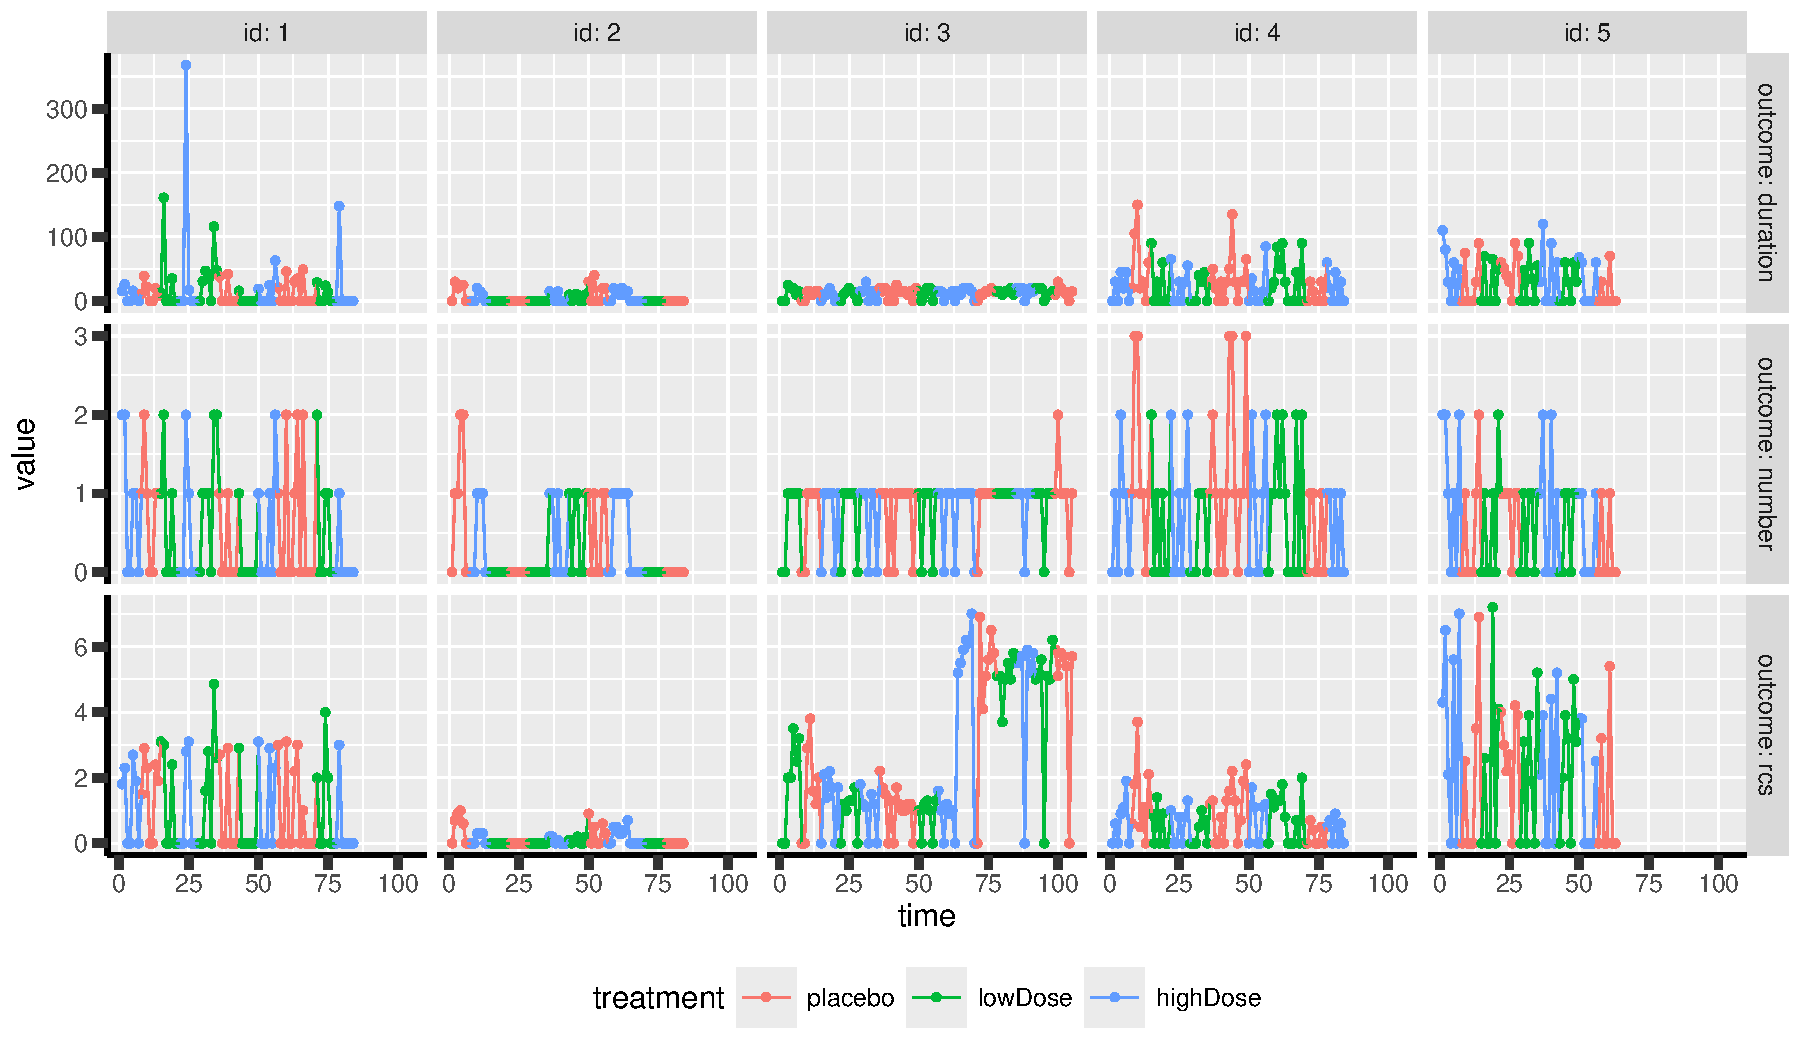
\includegraphics[trim={0 0 0 0},width=1\textwidth]{./figures/spaghetti-Nof1.pdf}
\end{center}
\subsection{With 2 treatment groups}
\label{sec:orgd7505e1}

\noindent Since \texttt{BuyseTest} can only handle two treatment group, we restrict the
dataset to placebo and low dose:
\begin{lstlisting}[language=r,numbers=none]
lowProfil <- profil[profil$treatment %in% c("placebo","lowDose"),]
lowProfil$treatment <- droplevels(lowProfil$treatment)
\end{lstlisting}

We will use the following hierarchy and threshold of clinical
relevance:
\begin{lstlisting}[language=r,numbers=none]
fff <- treatment ~ cont(rcs, threshold = 1.45, operator = "<0") + cont(number, threshold = 0.35, operator = "<0") + cont(duration, threshold = 3, operator = "<0")
\end{lstlisting}

\noindent One could either run a separate GPC for each patient:
\begin{lstlisting}[language=r,numbers=none]
ls.lowGPC <- by(lowProfil, lowProfil$id, BuyseTest, formula = fff, trace = FALSE)
df.lowGPC <- data.frame(do.call(rbind,lapply(ls.lowGPC, coef)),
                        do.call(rbind,lapply(ls.lowGPC, nobs)),
                        Buyse = as.numeric(NA), CMH = as.numeric(NA))
df.lowGPC$Buyse <- with(df.lowGPC, pairs/sum(pairs))
df.lowGPC$CMH <- with(df.lowGPC, (pairs/(placebo+lowDose))/sum(pairs/(placebo+lowDose)))
head(df.lowGPC)
\end{lstlisting}

\phantomsection
\label{}
\begin{verbatim}
     rcs_t1.45 number_t0.35  duration_t3 placebo lowDose pairs      Buyse       CMH
1 -0.016581633 -0.015306122 -0.021683673      28      28   784 0.04694049 0.0364368
2  0.000000000  0.153061224  0.183673469      28      28   784 0.04694049 0.0364368
3 -0.001632653  0.003265306 -0.008979592      35      35  1225 0.07334451 0.0455460
4  0.117346939  0.225765306  0.154336735      28      28   784 0.04694049 0.0364368
5 -0.043083900 -0.047619048 -0.029478458      21      21   441 0.02640402 0.0273276
6  0.102040816  0.092970522  0.077097506      21      21   441 0.02640402 0.0273276
\end{verbatim}


\noindent and pool the patient-specific Net Treatment
Benefits. Different weighting scheme are possible, e.g. same weight
for all patients, weight dependent on the number of blocks experienced
by the patient:
\begin{lstlisting}[language=r,numbers=none]
rbind(average = colMeans(df.lowGPC[,1:3]),
      Buyse = apply(df.lowGPC[,1:3], 2, weighted.mean, w = df.lowGPC$Buyse),
      CMH = apply(df.lowGPC[,1:3], 2, weighted.mean, w = df.lowGPC$CMH))
\end{lstlisting}

\phantomsection
\label{}
\begin{verbatim}
         rcs_t1.45 number_t0.35 duration_t3
average 0.02741742   0.02755903  0.03397497
Buyse   0.01628547   0.03730092  0.04215064
CMH     0.02145018   0.03266743  0.03869945
\end{verbatim}


This can be replicated using a single call to \texttt{BuyseTest} specifying a
strata in the formula:
\begin{lstlisting}[language=r,numbers=none]
lowGPC <- BuyseTest(update(fff, . ~ . + strata(id, match = TRUE)),
                    data = lowProfil, trace = FALSE)
confint(lowGPC)
\end{lstlisting}

\phantomsection
\label{}
\begin{verbatim}
estimate         se    lower.ci   upper.ci null   p.value
rcs_t1.45    0.02741742 0.02047690 -0.01273920 0.06748574    0 0.1808076
number_t0.35 0.02755903 0.03139999 -0.03401048 0.08892015    0 0.3803606
duration_t3  0.03397497 0.02801978 -0.02099009 0.08873527    0 0.2256649
\end{verbatim}


By default, equal weights are given to each patient but other
weighting schemes can be used by specifying the \texttt{pool.strata} argument:
\begin{lstlisting}[language=r,numbers=none]
lowGPC_Buyse <- BuyseTest(update(fff, . ~ . + strata(id, match = TRUE)),
                          data = lowProfil, pool.strata = "Buyse", trace = FALSE)
confint(lowGPC_Buyse)
\end{lstlisting}

\phantomsection
\label{}
\begin{verbatim}
estimate         se     lower.ci   upper.ci null    p.value
rcs_t1.45    0.01628547 0.01771680 -0.018444486 0.05097618    0 0.35807018
number_t0.35 0.03730092 0.02668638 -0.015057839 0.08945568    0 0.16257765
duration_t3  0.04215064 0.02400508 -0.004957166 0.08907178    0 0.07946061
\end{verbatim}


\begin{lstlisting}[language=r,numbers=none]
lowGPC_CMH <- BuyseTest(update(fff, . ~ . + strata(id, match = TRUE)),
                        data = lowProfil, pool.strata = "CMH", trace = FALSE)
confint(lowGPC_CMH)
\end{lstlisting}

\phantomsection
\label{}
\begin{verbatim}
estimate         se    lower.ci   upper.ci null   p.value
rcs_t1.45    0.02145018 0.01855984 -0.01493878 0.05778241    0 0.2479363
number_t0.35 0.03266743 0.02784903 -0.02195881 0.08709921    0 0.2411232
duration_t3  0.03869945 0.02491698 -0.01019050 0.08740482    0 0.1207617
\end{verbatim}


\begin{description}
\item[{\Warning}] in all approaches, all pairwise comparisons are performed within each patient, not only within-block comparisons.
\end{description}

In term of uncertainty quantification, it is important to specify
\texttt{match=TRUE} when using a single call so \texttt{BuyseTest} does not treat
each line of the dataset as an independent replicate. An intuitive way
to evaluate the standard error of the pooled estimator is to use the
across subject variability:
\begin{lstlisting}[language=r,numbers=none]
sqrt(apply(df.lowGPC[,1:3],2,var)/NROW(df.lowGPC))
\end{lstlisting}

\phantomsection
\label{}
\begin{verbatim}
 rcs_t1.45 number_t0.35  duration_t3 
0.02075177   0.03182148   0.02839590
\end{verbatim}


\noindent This is, up to a factor \texttt{N/(N-1)} exactly what the single call
approach returns. Actually we can retrieve this value by modifying the default options:
\begin{lstlisting}[language=r,numbers=none]
BuyseTest.options(order.Hprojection = 2)
lowGPC2 <- BuyseTest(update(fff, . ~ . + strata(id, match = TRUE)),
                     data = lowProfil, trace = FALSE)
confint(lowGPC2)
\end{lstlisting}

\phantomsection
\label{}
\begin{verbatim}
estimate         se    lower.ci   upper.ci null   p.value
rcs_t1.45    0.02741742 0.02075177 -0.01327825 0.06802241    0 0.1866527
number_t0.35 0.02755903 0.03182148 -0.03483625 0.08974030    0 0.3867027
duration_t3  0.03397497 0.02839590 -0.02172779 0.08946745    0 0.2318709
\end{verbatim}


\noindent  Similarly when using other weighting scheme. For instance we can
retrieve the results of the Buyse pooling scheme doing:
\begin{lstlisting}[language=r,numbers=none]
df.lowGPC_center <- sweep(df.lowGPC[,1:3], MARGIN = 2, FUN = "-", STATS = coef(lowGPC_Buyse))
df.lowGPC_Wcenter <- sweep(df.lowGPC_center, MARGIN = 1, FUN = "*", STATS = df.lowGPC$Buyse)
sqrt(colSums(df.lowGPC_Wcenter^2))
\end{lstlisting}

\phantomsection
\label{}
\begin{verbatim}
rcs_t1.45 number_t0.35  duration_t3 
  0.01771680   0.02668638   0.02400508
\end{verbatim}


\clearpage
\subsection{With 3 or more treatment groups (WORK IN PROGRESS!)}
\label{sec:org6db1537}

Handling more than two treatment groups is still an area of
development for the BuyseTest package. Several approaches have been
proposed in the litterature and here we focus on one that aim at
handling the non-transitivity issues that comes with Wilcoxon-like
tests \citep{lumley2016characterising}. This approach compare the
treatment-specific distribution to a pooled distribution over all
treatment groups \citep{thangavelu2007wilcoxon}:

\begin{lstlisting}[language=r,numbers=none]
CasinoTest(update(fff, . ~ . + strata(id)), data = profil,
           method.inference = "none", type = "unweighted")
## do not trust inference since it would require accounting for matching
\end{lstlisting}

\phantomsection
\label{}
\begin{verbatim}
                   endpoint treatment     estimate se lower.ci upper.ci null p.value
placebo: rcs            rcs   placebo -0.012193158 NA       NA       NA   NA      NA
lowDose: rcs            rcs   lowDose  0.008015351 NA       NA       NA   NA      NA
highDose: rcs           rcs  highDose  0.004177807 NA       NA       NA   NA      NA
placebo: number      number   placebo -0.020434169 NA       NA       NA   NA      NA
lowDose: number      number   lowDose  0.011566310 NA       NA       NA   NA      NA
highDose: number     number  highDose  0.008867860 NA       NA       NA   NA      NA
placebo: duration  duration   placebo -0.024148505 NA       NA       NA   NA      NA
lowDose: duration  duration   lowDose  0.013113939 NA       NA       NA   NA      NA
highDose: duration duration  highDose  0.011034566 NA       NA       NA   NA      NA
\end{verbatim}

Its main drawback is that the assessment of say \texttt{placebo}
vs. \texttt{lowDose} is now influenced by \texttt{highDose}.
\section*{References}
\label{sec:orgc4ca38e}
\begingroup
\renewcommand{\section}[2]{}

\bibliographystyle{apalike}
\bibliography{bibliography}

\endgroup
\end{document}
